\section{Evaluation}
\label{section:evaluation}

All tests were performed on the Franklin Cray-XT4 supercomputer\cite{franklin}
located at NERSC\cite{NERSC}.  The Franklin supercomputer features 9,572
Opteron 2.3 gigahertz quad core processors with 2 gigabytes of memory per
core.  Its Lustre parallel file system supports a theoretical peak of 16
gigabytes/second to each of two /scratch file systems.

In order to evaluate the scalability of our subsetter we performed strong
scaling tests.  The performance data collected was generated by custom
wrappers to the functions we developed.  The IO wrappers perform barriers
before and after each collective IO operation is called with the start and end
timestamps collected immediately after each barrier using
\verb=clock_gettime()= or \verb=gettimeofday()= depending on platform
availability.  Before program termination, the number of bytes written and
read and the total time spent performing IO is collected on the zeroth process
and displayed in terms of Gigabytes/second.  The profiling information
collects the number of times each function is called and how much time was
spent in each function.  It is only reported for the zeroth process and is
meant as a general measure of performance.  The IO and profile data were
collected on separate runs so that the collection of the former (with
additional barriers) would not affect the latter.  This test was run over 24
timesteps of an edge variable at a 4 kilometer resolution ($R=11$) specifying
a subset region of the Madden-Julien Oscillation\cite{MJO}
(20N,-20S,160E,90E).  The MJO region is roughly 6.5\% of the global data.  One
timestep of the edge variable is 12.1875 GB.  The number of processors was
doubled each run starting from 64 through 2048.

Two versions of the subsetter were originally tested, one to test the
subsetter as a whole and the the other to test the algorithms by turning off
nearly all IO.  (Reading of the grid topology was still required resulting in
an insubstantial amount of IO.)  Turning off the IO is important in order to
evaluate the scalability of our packing algorithms.  Since our current
software does not involve any algebraic operations, this case is also an
accurate representation of communication.

After the initial tests were performed, it was noted that the majority of data
being read was discarded.  An optimized version of the subsetter was developed
which determines ahead of time which processes will not participate in the
subset operation.  This allowed for the nonparticipating processes to specify
empty regions in the collective read operation, reducing the total amount of
data read prior to the subset.  It was important to show test results for both
the original and optimized versions of the subsetter in order to illustrate
the need for efficient IO algorithms as well as to accurately capture the IO
requirements when reading the entire horizontal region of data.

Fig. \ref{fig:strong} shows the timing results of the tests.  Three versions
of the code were run.  "Subsetter" represents the original program,
"Optimized" represents our optimized read, and "Algorithms" represents
executing with nearly all IO turned off.  Comparing the original subsetter to
the algorithms case, clearly, IO represents a significant portion of the
execution time.  As the number of cores increases, the optimized case more
closely resembles the alrogithms alone.  The benefit of additional processors
appears to have reached a plateau near 1024 processors for all cases, however
this may be due to the size of the problem since run times at this scale are
only a few minutes in length.

\begin{figure}[!t]
\center
\resizebox{3.5in}{!}{
% GNUPLOT: LaTeX picture with Postscript
\begingroup
  \makeatletter
  \providecommand\color[2][]{%
    \GenericError{(gnuplot) \space\space\space\@spaces}{%
      Package color not loaded in conjunction with
      terminal option `colourtext'%
    }{See the gnuplot documentation for explanation.%
    }{Either use 'blacktext' in gnuplot or load the package
      color.sty in LaTeX.}%
    \renewcommand\color[2][]{}%
  }%
  \providecommand\includegraphics[2][]{%
    \GenericError{(gnuplot) \space\space\space\@spaces}{%
      Package graphicx or graphics not loaded%
    }{See the gnuplot documentation for explanation.%
    }{The gnuplot epslatex terminal needs graphicx.sty or graphics.sty.}%
    \renewcommand\includegraphics[2][]{}%
  }%
  \providecommand\rotatebox[2]{#2}%
  \@ifundefined{ifGPcolor}{%
    \newif\ifGPcolor
    \GPcolortrue
  }{}%
  \@ifundefined{ifGPblacktext}{%
    \newif\ifGPblacktext
    \GPblacktexttrue
  }{}%
  % define a \g@addto@macro without @ in the name:
  \let\gplgaddtomacro\g@addto@macro
  % define empty templates for all commands taking text:
  \gdef\gplbacktext{}%
  \gdef\gplfronttext{}%
  \makeatother
  \ifGPblacktext
    % no textcolor at all
    \def\colorrgb#1{}%
    \def\colorgray#1{}%
  \else
    % gray or color?
    \ifGPcolor
      \def\colorrgb#1{\color[rgb]{#1}}%
      \def\colorgray#1{\color[gray]{#1}}%
      \expandafter\def\csname LTw\endcsname{\color{white}}%
      \expandafter\def\csname LTb\endcsname{\color{black}}%
      \expandafter\def\csname LTa\endcsname{\color{black}}%
      \expandafter\def\csname LT0\endcsname{\color[rgb]{1,0,0}}%
      \expandafter\def\csname LT1\endcsname{\color[rgb]{0,1,0}}%
      \expandafter\def\csname LT2\endcsname{\color[rgb]{0,0,1}}%
      \expandafter\def\csname LT3\endcsname{\color[rgb]{1,0,1}}%
      \expandafter\def\csname LT4\endcsname{\color[rgb]{0,1,1}}%
      \expandafter\def\csname LT5\endcsname{\color[rgb]{1,1,0}}%
      \expandafter\def\csname LT6\endcsname{\color[rgb]{0,0,0}}%
      \expandafter\def\csname LT7\endcsname{\color[rgb]{1,0.3,0}}%
      \expandafter\def\csname LT8\endcsname{\color[rgb]{0.5,0.5,0.5}}%
    \else
      % gray
      \def\colorrgb#1{\color{black}}%
      \def\colorgray#1{\color[gray]{#1}}%
      \expandafter\def\csname LTw\endcsname{\color{white}}%
      \expandafter\def\csname LTb\endcsname{\color{black}}%
      \expandafter\def\csname LTa\endcsname{\color{black}}%
      \expandafter\def\csname LT0\endcsname{\color{black}}%
      \expandafter\def\csname LT1\endcsname{\color{black}}%
      \expandafter\def\csname LT2\endcsname{\color{black}}%
      \expandafter\def\csname LT3\endcsname{\color{black}}%
      \expandafter\def\csname LT4\endcsname{\color{black}}%
      \expandafter\def\csname LT5\endcsname{\color{black}}%
      \expandafter\def\csname LT6\endcsname{\color{black}}%
      \expandafter\def\csname LT7\endcsname{\color{black}}%
      \expandafter\def\csname LT8\endcsname{\color{black}}%
    \fi
  \fi
  \setlength{\unitlength}{0.0500bp}%
  \begin{picture}(7200.00,5040.00)%
    \gplgaddtomacro\gplbacktext{%
      \csname LTb\endcsname%
      \put(990,660){\makebox(0,0)[r]{\strut{} 0}}%
      \put(990,1073){\makebox(0,0)[r]{\strut{} 100}}%
      \put(990,1487){\makebox(0,0)[r]{\strut{} 200}}%
      \put(990,1900){\makebox(0,0)[r]{\strut{} 300}}%
      \put(990,2313){\makebox(0,0)[r]{\strut{} 400}}%
      \put(990,2727){\makebox(0,0)[r]{\strut{} 500}}%
      \put(990,3140){\makebox(0,0)[r]{\strut{} 600}}%
      \put(990,3553){\makebox(0,0)[r]{\strut{} 700}}%
      \put(990,3967){\makebox(0,0)[r]{\strut{} 800}}%
      \put(990,4380){\makebox(0,0)[r]{\strut{} 900}}%
      \put(1937,440){\makebox(0,0){\strut{}64}}%
      \put(2752,440){\makebox(0,0){\strut{}128}}%
      \put(3567,440){\makebox(0,0){\strut{}256}}%
      \put(4381,440){\makebox(0,0){\strut{}512}}%
      \put(5196,440){\makebox(0,0){\strut{}1024}}%
      \put(6011,440){\makebox(0,0){\strut{}2048}}%
      \put(220,2520){\rotatebox{90}{\makebox(0,0){\strut{}Time (seconds)}}}%
      \put(3974,110){\makebox(0,0){\strut{}Cores}}%
      \put(3974,4710){\makebox(0,0){\strut{}Strong Scaling Test}}%
    }%
    \gplgaddtomacro\gplfronttext{%
      \csname LTb\endcsname%
      \put(5839,4207){\makebox(0,0)[r]{\strut{}Subsetter}}%
      \csname LTb\endcsname%
      \put(5839,3987){\makebox(0,0)[r]{\strut{}Algorithms}}%
    }%
    \gplbacktext
    \put(0,0){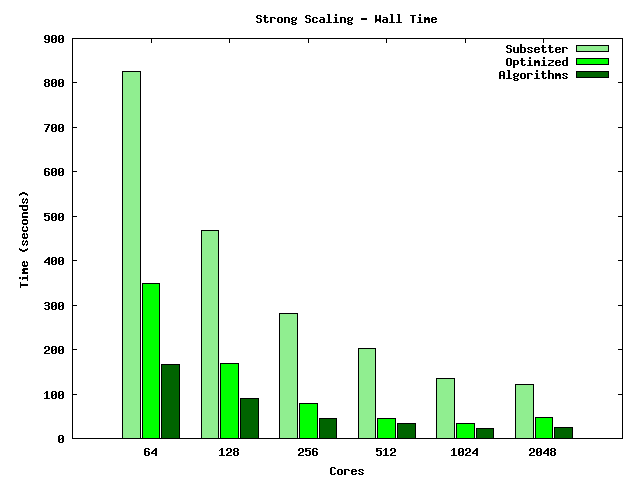
\includegraphics{strong_hist}}%
    \gplfronttext
  \end{picture}%
\endgroup

}
\caption{Strong Scaling Test.  First, the subsetter was run as a whole
program ("Subsetter").  Second, the subsetter was optimized to read less data
in the case of a subset ("Optimized").  Lastly, nearly all IO was stripped
from the program to capture the performance of the packing routines
("Algorithms").  At smaller numbers of cores, there is a greater difference
between time spent in IO and time spent everywhere else.}
\label{fig:strong}
\end{figure}

Fig. \ref{fig:strong_io} shows the IO bandwidth results of the test.  This
test captures the scalability of the IO system which correlates with the
scalability portrayed in Fig. \ref{fig:strong}.  Although in the unoptimized
case the read bandwidth may have benefited from additional cores beyond 2048,
the write bandwidth appears to have reached a plateau near 1024 processors.
The hardware is likely reaching its saturation point if not already there.
The optimized bandwidths matched those of the original subsetter given a small
amount of variability.  The notable exception is that of the optimized read
bandwidth which leveled off near 512 cores.

\begin{figure}[!t]
\center
\resizebox{3.5in}{!}{
% GNUPLOT: LaTeX picture with Postscript
\begingroup
  \makeatletter
  \providecommand\color[2][]{%
    \GenericError{(gnuplot) \space\space\space\@spaces}{%
      Package color not loaded in conjunction with
      terminal option `colourtext'%
    }{See the gnuplot documentation for explanation.%
    }{Either use 'blacktext' in gnuplot or load the package
      color.sty in LaTeX.}%
    \renewcommand\color[2][]{}%
  }%
  \providecommand\includegraphics[2][]{%
    \GenericError{(gnuplot) \space\space\space\@spaces}{%
      Package graphicx or graphics not loaded%
    }{See the gnuplot documentation for explanation.%
    }{The gnuplot epslatex terminal needs graphicx.sty or graphics.sty.}%
    \renewcommand\includegraphics[2][]{}%
  }%
  \providecommand\rotatebox[2]{#2}%
  \@ifundefined{ifGPcolor}{%
    \newif\ifGPcolor
    \GPcolortrue
  }{}%
  \@ifundefined{ifGPblacktext}{%
    \newif\ifGPblacktext
    \GPblacktexttrue
  }{}%
  % define a \g@addto@macro without @ in the name:
  \let\gplgaddtomacro\g@addto@macro
  % define empty templates for all commands taking text:
  \gdef\gplbacktext{}%
  \gdef\gplfronttext{}%
  \makeatother
  \ifGPblacktext
    % no textcolor at all
    \def\colorrgb#1{}%
    \def\colorgray#1{}%
  \else
    % gray or color?
    \ifGPcolor
      \def\colorrgb#1{\color[rgb]{#1}}%
      \def\colorgray#1{\color[gray]{#1}}%
      \expandafter\def\csname LTw\endcsname{\color{white}}%
      \expandafter\def\csname LTb\endcsname{\color{black}}%
      \expandafter\def\csname LTa\endcsname{\color{black}}%
      \expandafter\def\csname LT0\endcsname{\color[rgb]{1,0,0}}%
      \expandafter\def\csname LT1\endcsname{\color[rgb]{0,1,0}}%
      \expandafter\def\csname LT2\endcsname{\color[rgb]{0,0,1}}%
      \expandafter\def\csname LT3\endcsname{\color[rgb]{1,0,1}}%
      \expandafter\def\csname LT4\endcsname{\color[rgb]{0,1,1}}%
      \expandafter\def\csname LT5\endcsname{\color[rgb]{1,1,0}}%
      \expandafter\def\csname LT6\endcsname{\color[rgb]{0,0,0}}%
      \expandafter\def\csname LT7\endcsname{\color[rgb]{1,0.3,0}}%
      \expandafter\def\csname LT8\endcsname{\color[rgb]{0.5,0.5,0.5}}%
    \else
      % gray
      \def\colorrgb#1{\color{black}}%
      \def\colorgray#1{\color[gray]{#1}}%
      \expandafter\def\csname LTw\endcsname{\color{white}}%
      \expandafter\def\csname LTb\endcsname{\color{black}}%
      \expandafter\def\csname LTa\endcsname{\color{black}}%
      \expandafter\def\csname LT0\endcsname{\color{black}}%
      \expandafter\def\csname LT1\endcsname{\color{black}}%
      \expandafter\def\csname LT2\endcsname{\color{black}}%
      \expandafter\def\csname LT3\endcsname{\color{black}}%
      \expandafter\def\csname LT4\endcsname{\color{black}}%
      \expandafter\def\csname LT5\endcsname{\color{black}}%
      \expandafter\def\csname LT6\endcsname{\color{black}}%
      \expandafter\def\csname LT7\endcsname{\color{black}}%
      \expandafter\def\csname LT8\endcsname{\color{black}}%
    \fi
  \fi
  \setlength{\unitlength}{0.0500bp}%
  \begin{picture}(7200.00,5040.00)%
    \gplgaddtomacro\gplbacktext{%
      \csname LTb\endcsname%
      \put(726,660){\makebox(0,0)[r]{\strut{} 0}}%
      \put(726,1336){\makebox(0,0)[r]{\strut{} 1}}%
      \put(726,2013){\makebox(0,0)[r]{\strut{} 2}}%
      \put(726,2689){\makebox(0,0)[r]{\strut{} 3}}%
      \put(726,3365){\makebox(0,0)[r]{\strut{} 4}}%
      \put(726,4042){\makebox(0,0)[r]{\strut{} 5}}%
      \put(1711,440){\makebox(0,0){\strut{}64}}%
      \put(2563,440){\makebox(0,0){\strut{}128}}%
      \put(3416,440){\makebox(0,0){\strut{}256}}%
      \put(4268,440){\makebox(0,0){\strut{}512}}%
      \put(5121,440){\makebox(0,0){\strut{}1024}}%
      \put(5973,440){\makebox(0,0){\strut{}2048}}%
      \put(220,2520){\rotatebox{90}{\makebox(0,0){\strut{}Gigabytes/second}}}%
      \put(3842,110){\makebox(0,0){\strut{}Cores}}%
      \put(3842,4710){\makebox(0,0){\strut{}Strong Scaling - IO - 48 OSTs}}%
    }%
    \gplgaddtomacro\gplfronttext{%
      \csname LTb\endcsname%
      \put(5839,4207){\makebox(0,0)[r]{\strut{}Read}}%
      \csname LTb\endcsname%
      \put(5839,3987){\makebox(0,0)[r]{\strut{}Write}}%
    }%
    \gplbacktext
    \put(0,0){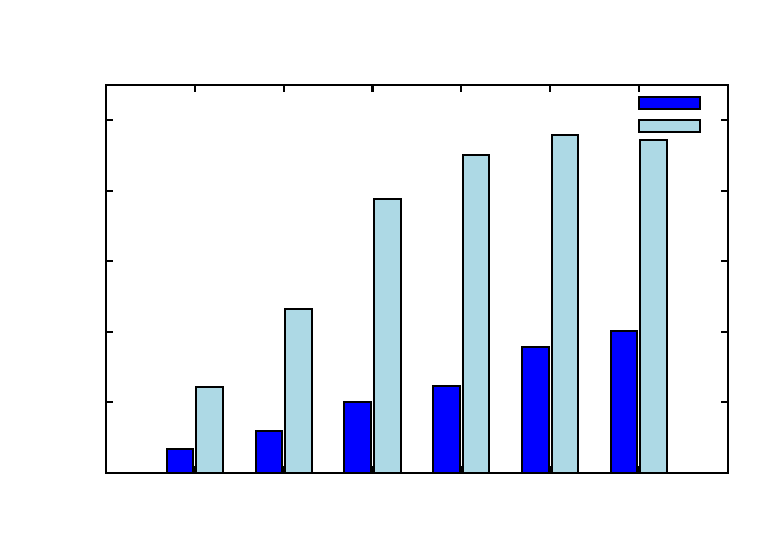
\includegraphics{strong_io_hist}}%
    \gplfronttext
  \end{picture}%
\endgroup

}
\caption{Strong Scaling Test for IO Bandwidth.  The Read and Write bandwidths
are compared as the number of cores are increased.  The subsetter and its
optimized versions are both shown.  In general, all bandwidths increased with
respect to the number of cores.  The optimized bandwidths matched those of the
original subsetter given a small amount of variability.  The notable exception
is that of the optimized read bandwidth which leveled off near 512 cores.}
\label{fig:strong_io}
\end{figure}

Table \ref{tab:strong_prof} represents a profile for process zero for the 2048
process run.  The function names are sufficiently self-documenting for those
familiar with C++ syntax.  The zeroth process represents a worst-case scenario
since the default distribution of data using GA will always put data on at
least the zeroth process implying process zero should have at least as much
work to perform as any other processor.  The profile for the 2048 run was
selected arbitrarily, however the profiles for the other strong scaling runs
(not shown) demonstrated a similar trend.  The functions which did not
contribute a significant amount of time to the program were removed and the
table is sorted by total time spent in the function.  The number of calls to
the read and write routines were small.  (Not shown in Table
\ref{tab:strong_prof} is the number of calls to the function comparing each
latitude/longitude pair to the desired subset region which accounts for over
60\% of the function calls.)  However, the amount of time spent in the read
and write routines was significant.  In all cases, the amount of time spent in
IO was at least 75\% of the program's execution.  IO is clearly the dominant
factor in running our code.

\begin{table*}[!t]
\center
\caption{Partial Profile for Process 0 at 2048 Cores - MJO Region}
\label{tab:strong_prof}
\begin{tabular}{lrrrrrr}
Name&Calls&Percent Calls&Time (seconds)&Percent Time&Time/call (seconds)\\
NetcdfVariable::read()                    &39&0.1&156.1&93.0&4.00\\
NetcdfFileWriter::write(int,int,int)      &34&0.1&  5.9& 3.5&0.17\\
VariableDecorator::read()                 & 5&0.0&  1.7& 1.0&0.34\\
NetcdfDataset::NetcdfDataset(string)      & 5&0.0&  1.2& 0.7&0.24\\
Dataset::adjust\_masks(LatLonBox)         & 1&0.0&  1.0& 0.6&1.05\\
ConnectivityVariable::reindex()           & 3&0.0&  0.7& 0.4&0.25\\
NetcdfFileWriter::NetcdfFileWriter(string)& 1&0.0&  0.2& 0.2&0.29\\
\end{tabular}
\end{table*}

Table \ref{tab:strong_prof_opt} represents a profile for process zero for
the 2048 process run using the optimized subsetter.  The notable differences
between Table \ref{tab:strong_prof_opt} and Table \ref{tab:strong_prof} are
the total time and percentage of time spent in each function.  Although the
optimized subsetter spends substantially less time reading, the majority of
time is still spent in IO.  Although still dominant, IO is a less significant
contributer to the total execution time.

\begin{table*}[!t]
\center
\caption{Partial Profile for Process 0 at 2048 Cores - MJO Region - Optimized}
\label{tab:strong_prof_opt}
\begin{tabular}{lrrrrrr}
Name&Calls&Percent Calls&Time (seconds)&Percent Time&Time/call (seconds)\\
NetcdfVariable::read()                    & 39&0.1&22.8&65.4&0.58\\
NetcdfFileWriter::write(int,int,int)      & 34&0.1& 6.5&18.7&0.19\\
NetcdfDataset::NetcdfDataset(string)      &  5&0.0& 1.2& 3.4&0.24\\
VariableDecorator::read()                 &  5&0.0& 1.1& 3.0&0.21\\
Dataset::adjust\_masks(LatLonBox)         &  1&0.0& 0.8& 2.4&0.82\\
ConnectivityVariable::reindex()           &  3&0.0& 0.8& 2.2&0.26\\
NetcdfFileWriter::NetcdfFileWriter(string)&  1&0.0& 0.4& 1.1&0.37\\
\end{tabular}
\end{table*}

\subsection{Discussion}

Running our subsetter at a scale of over 2000 cores is initially promising.
Fig. \ref{fig:strong} demonstrates that the algorithms we developed scale
regardless of the time spent in IO.  The performance of the original subsetter
can be considered as the case where global operations are performed such that
subset operations are not needed.  These global operations will stress the IO
system the greatest.  The optimized subsetter will not help in cases of global
operations. 

The global profile in Table \ref{tab:strong_prof} suggests that IO accounts
for nearly 95\% of program execution at 2048 cores.  This is not a stretch of
the imagination since our software reads, subsets, and then writes.  Even if
our code performed a significant calculation after each read of the edge
variable, the profile would likely remain IO bound but less so.  At fewer
numbers of cores the percentage of time spent in IO ranged from 75\% to the
95\% shown in Table \ref{tab:strong_prof}.  Even in the optimized case, the
profile remains IO bound.

The reason for the disproportionately faster write bandwidth versus read
bandwith seen in Fig. \ref{fig:strong_io} is likely due to caching by the
Lustre parallel filesystem.  The relatively small amount of data being written
is likely being copied to an internal buffer allowing the functions to return
rather quickly.
